% Intended LaTeX compiler: pdflatex
\documentclass[10pt,a4paper,UTF8]{article}
\usepackage{zclorg}
\usepackage{tikztheorem}
\author{zcl.space}
\date{}
\title{强大数定理}
\hypersetup{
 pdfauthor={zcl.space},
 pdftitle={强大数定理},
 pdfkeywords={probability},
 pdfsubject={},
 pdfcreator={Emacs 25.0.50.1 (Org mode 9.0.6)},
 pdflang={English}}
\begin{document}

\maketitle
\tableofcontents
\titlepic{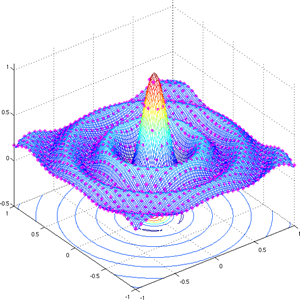
\includegraphics[scale=0.25]{../../img/sinc.PNG}}
强大数定理是概率论中最广为人知的结果。它表明了独立同分布随机变量序列的均值以概率1收敛到分布的均值。

\begin{tikztheorem}
设\(X_{1},X_{2},\ldots\)为以独立同分布随机变量序列,其公共均值为\(\mu = E[X_{i}]\)有限,则下式以概率1成立:
\begin{equation}
\label{eq:1}
\frac{X_{1} + X_{2} + \ldots +X_{n}}{n} \to \mu \qquad n\to \infty
\end{equation}
\end{tikztheorem}
作为强大数定理的一个应用,设有一独立重复试验,令\(E\)为某一事件,\(P(E)\)为事件\(E\)发生的概率,又令:
\begin{equation}
\label{eq:2}
X_{i} =
\begin{cases}
1 & \mathrm{E\quad occurs} \\
0 & \mathrm{others}
\end{cases}
\end{equation}
根据强大数定理,以概率\(1\),有:
\begin{equation}
\label{eq:3}
\frac{X_{1} + X_{2} + \ldots +X_{n}}{n} \to E[X] = P(E)
\end{equation}

因为\(X_{1}+\ldots +X_{n}\)表示在前\(n\)次试验中事件\(E\)发生的次数,因此式 (\ref{eq:3})说明事件\(E\)在前\(n\)次试验中发生的频率以概率\(1\)收敛到它的概率\(P(E)\)。

在强大数定理的证明中我们假设\(X_{i}\)具有有限\(e\)阶矩,即假定\(E[X_{i}^{4}] = K < \infty\),但在没有这个假设的条件下定理仍可以被证明。

\begin{proof}
首先假定\(E[X_{i}] = \mu = 0\),记\(S_{n} = \sum_{i=1}^{n}X_{i}\),考虑:
\begin{equation}
\label{eq:4}
E[S_{n}^{4}] = E[(X_{1} + \ldots +X_{n})(X_{1} + \ldots + X_{n})\times (X_{1}+\ldots +X_{n})(X_{1}+ \ldots + X_{n})]
\end{equation}
将上式右边期望展开,得到各项之和,这些项具有的形式为:
\begin{equation}
\label{eq:5}
X_{i}^{4} \qquad X_{i}^{3}X_{j} \qquad X_{i}^{2}X_{j}^{2} \qquad X_{i}^{2}X_{j}X_{k} \qquad X_{i}X_{j}X_{k}X_{l}
\end{equation}
其中\(i,j,k,l\)各不相同。由于\(E[X_{i}] = 0\),利用独立性有:
\begin{eqnarray}
\label{eq:6}
E[X_{i}^{3}X_{j}] &=& 0\\
E[X_{i}^{2}X_{j}X_{k}] &=& 0 \\
E[X_{i}X_{j}X_{k}X_{l}] &=& 0
\end{eqnarray}
在展开式中\(X_{i}^{4}\)的系数为1,故在\(E[S_{n}^{4}]\)中可将所有\(X_{i}^{4}\)的期望合并成\(nE[X_{i}^{4}]\),对固定的\(i,j\),\(S_{n}^{4}\)的展开式中\(X_{i}^{2}X_{j}^{2}\)一共有\(\binom{4}{2}= 6\)项,因此,\(S_{n}^{4}\)的展开式中与\(X_{i}^{2}X_{j}^{2}\)有关的部分为\(6\sum_{i < j}X_{i}^{2}X_{j}^{2}\),其中求和号是对\(\{1,2,\ldots ,n\}\)的所有量元素组求和。因此,它的期望为\(6\binom{n}{2}E[X_{i}^{2}X_{j}^{2}]\),这样:
\begin{equation}
\label{eq:7}
E[S_{n}^{4}] = nE[X_{i}^{4}] + 6\binom{n}{2}E[X_{i}^{2}X_{j}^{2}] = nK + 3n(n-1)E[X_{i}^{2}]E[X_{j}^{2}]
\end{equation}

又因为:
\begin{equation}
\label{eq:8}
0 \leq \mathrm{Var}(X_{i}^{2}) = E[X_{i}^{4}] - (E[X_{i}^{2}])^{2}
\end{equation}
我们有:
\begin{equation}
\label{eq:9}
(E[X_{i}^{2}]) \leq E[X_{i}^{4}] = K
\end{equation}
综上,有:
\begin{equation}
\label{eq:10}
E[S_{n}^{4}] \leq nK + 3n(n-1)K
\end{equation}
从而:
\begin{equation}
\label{eq:11}
E[\frac{S_{n}^{4}}{n^{4}}] \leq \frac{K}{n^{3}} + \frac{3K}{n^{2}}
\end{equation}
因此:
\begin{equation}
\label{eq:12}
E[\sum_{n=1}^{\infty}\frac{S_{n}^{4}}{n^{4}}] = \sum_{n=1}^{\infty}E[\frac{S_{n}^{4}}{n^{4}}] < \infty
\end{equation}
即随机变量\(\sum_{n=1}^{\infty}S_{n}^{4}/n^{4}\)的期望有限,说明以概率\(1\)有\(\sum_{n=1}^{\infty}S_{n}^{4}/n^{4} < \infty\),进而有:
\begin{equation}
\label{eq:13}
\lim_{n\to \infty}\frac{S_{n}^{4}}{n^{4}} = 0
\end{equation}
如果\(S_{n}^{4}/n^{4} = (S_{n}/n)^{4} \to 0\),那么一定有\(S_{n}/n \to 0\);因此,我们可以证明以概率\(1\),有:
\begin{equation}
\label{eq:14}
\frac{S_{n}}{n}\to 0 \qquad n\to \infty
\end{equation}
当\(\mu = E[X_{i}]\neq 0\)时,可以化为期望为\(0\)的情况来处理,由于\(E[X_{i} - \mu] = 0\),利用刚才得到的结论,可知以概率1有:
\begin{equation}
\label{eq:15}
\lim_{n\to \infty}\sum_{i=1}^{n}\frac{X_{i} - \mu}{n} = 0
\end{equation}
即以概率\(1\)有:
\begin{equation}
\label{eq:16}
\lim_{n\to\infty}\sum_{i=1}^{n}\frac{X_{i}}{n} = \mu
\end{equation}
\end{proof}
\end{document}
